%\documentclass[aspectratio=169, handout]{beamer}
\documentclass[aspectratio=169]{beamer}


\makeatletter
\renewcommand*\env@matrix[1][\arraystretch]{%
  \edef\arraystretch{#1}%
  \hskip -\arraycolsep
  \let\@ifnextchar\new@ifnextchar
  \array{*\c@MaxMatrixCols c}}
\makeatother

\usepackage{tikz}
\usetikzlibrary{tikzmark,fit,shapes.geometric}


\newcommand{\transp}{^{\rm{T}}}

\usepackage{cases}
\usepackage[english]{babel}
% or whatever
\usepackage{xcolor}
\usepackage{colortbl}
\usepackage[latin1]{inputenc}
\usepackage[super]{nth}
% or whatever
%\setbeamertemplate{footline}[page number]
\setbeamertemplate{footline}
        {
      \leavevmode%
      \hbox{%
      \begin{beamercolorbox}[wd=.333333\paperwidth,ht=2.25ex,dp=1ex,center]{author in head/foot}%
        \usebeamerfont{author in head/foot}\insertshortauthor%~~(\insertshortinstitute)
      \end{beamercolorbox}%
      \begin{beamercolorbox}[wd=.333333\paperwidth,ht=2.25ex,dp=1ex,center]{title in head/foot}%
        \usebeamerfont{title in head/foot}\insertshorttitle
      \end{beamercolorbox}%
      \begin{beamercolorbox}[wd=.333333\paperwidth,ht=2.25ex,dp=1ex,right]{date in head/foot}%
        \usebeamerfont{date in head/foot}\insertshortdate{}\hspace*{2em} \insertframenumber{}  \hspace*{2em}%/ \inserttotalframenumber\hspace*{2ex} 

    %#turning the next line into a comment, erases the frame numbers
        

      \end{beamercolorbox}}%
      \vskip 0pt%
    }

\usepackage{times}
\usepackage[T1]{fontenc}
\usepackage{psfrag}
\usepackage{algorithm}
\usepackage{amsmath}
\usepackage{amssymb}
\usepackage{tabularx}
\usepackage{algpseudocode}
\usepackage{mathrsfs}
\usepackage{textpos}
\usepackage{graphicx}
\usepackage{tcolorbox}
\usepackage{multicol}
\usepackage{tikz}
\usetikzlibrary{arrows.meta,shapes.arrows}
%\setkeys{Gin}{draft}
\usepackage{caption}
\captionsetup{font=scriptsize,labelfont=scriptsize}
\usepackage{color}
\DeclareCaptionFont{blue}{\color{blue}}
\captionsetup{labelfont=blue}
\usepackage{tikz}
\tikzset{
  every overlay node/.style={
    draw=white,anchor=north west,
  },
}
\def\checkmark{\tikz\fill[scale=0.4](0,.35) -- (.25,0) -- (1,.7) -- (.25,.15) -- cycle;}
\def\tikzoverlay{%
   \tikz[baseline,overlay]\node[every overlay node]
}%
%\DeclareGraphicsRule{.png}{png}{.png.bb}{}

\newtheorem{assumption}{Assumption} %jw

\newcommand{\T}{{\rm T}}

\newcommand\blfootnote[1]{%
  \begingroup
  \renewcommand\thefootnote{}\footnote{#1}%
  \addtocounter{footnote}{-1}%
  \endgroup
}
\setcounter{tocdepth}{1}
\beamertemplatenavigationsymbolsempty


\title[Lecture 9: Regression] % (optional, use only with long paper titles)
{Data, Environment and Society: \\{Lecture 9: Intro to regression}}


%\subtitle
%{Include Only If Paper Has a Subtitle}

\author[ER131: Data, Environment and Society] 
{Instructor: Duncan Callaway\\
GSI: Salma Elmallah} 
% - Give the names in the same order as the appear in the paper.
% - Use the \inst{?} command only if the authors have different
%   affiliation.

%\logo{
%\includegraphics[width=1.5cm,height=1.5cm,keepaspectratio]{uvic_logo_h.jpg}
%}
\vspace{-20mm}
\institute[UC Berkeley] % (optional, but mostly needed)
 {\small{ \bf September 26, 2019}}


\date[September 26, 2019]


\begin{document}

\begin{frame}[plain, noframenumbering]
  \titlepage
\end{frame}

\begin{frame}{Announcements}

\textbf{Today}
\begin{itemize}
\item Review bias-variance tradeoff
\item Regression
\begin{itemize}
	\item K-nearest neighbors
	\item Linear least squares
\end{itemize}
\end{itemize}

\textbf{Reading}
\begin{itemize}
\item Today's lecture draws from DS100 Ch10, ISLR Ch 2, ISLR Ch 3.1
\item For next week
\begin{itemize}
\item Read Alstone \textit{et al} for next Tuesday -- in class discussion
\item Review ISLR Ch 3.1-3.2
\end{itemize}
\end{itemize}

\end{frame}

\begin{frame}{Before moving on, a little linear algebra:}

Here are two vectors:  
\begin{align*}
\mathbf{a} =  
\begin{bmatrix} 
	a_1 \\
	a_2  
\end{bmatrix}\\
\mathbf{b}=
 \begin{bmatrix}
	b_1\\
	b_2
\end{bmatrix} 
\end{align*}

Then the ``dot'' product of the two vectors is

\begin{align*}
\mathbf{a}\cdot \mathbf{b} = a_1b_1 + a_2b_2
\end{align*}

\end{frame}


\begin{frame}{Next, a little more linear algebra:}

We can also multiply \textit{matrices} and vectors.  Matrices are like column vectors stacked side by side
\begin{align*}
\mathbf{A} =  
\begin{bmatrix} 
	a_{11} &a_{12}\\
	a_{21} &a_{22}
\end{bmatrix}
\end{align*}

Then matrix multiplication gives us
\begin{align*}
\mathbf{A}\mathbf{b} = 
\begin{bmatrix} 
	a_{11} &a_{12}\\
	a_{21} &a_{22}
\end{bmatrix}
\begin{bmatrix}
	b_1\\
	b_2
\end{bmatrix} 
=\begin{bmatrix}
	a_{11}b_1+a_{12}b_2 \\
	a_{21}b_1+a_{22}b_2  
\end{bmatrix} 
\end{align*}

\pause
Each element of the resulting matrix (or vector) is the dot product of a row of the first term ($\mathbf{A}$) and a column of the second ($\mathbf{b}$)

\vspace{5mm}
Therefore:   the horizontal ``dimension'' of the first must be the same as the vertical ``dimension'' of the second.

\end{frame}

\begin{frame}{Let's define matrices for our data:}


Suppose we have $n$ observations, $(x_i, y_i)$.  We'll arrange them all into a matrix form:

\begin{align*}
X = \begin{bmatrix} 
  1 & x_1\\
  1 & x_2\\
  \vdots & \vdots \\
  1 & x_n 
\end{bmatrix}, 
Y = 
\begin{bmatrix} 
  y_1\\
  y_2\\
   \vdots \\
  y_n 
\end{bmatrix} 
\end{align*}

Note: when we start working with more than one independent variable, $X$ will have a new column for each new variable.  

\end{frame}

\begin{frame}{And then a lot more linear algebra:}
Let's define the `transpose':
\begin{align*}
X = \begin{bmatrix} 
  1 & x_1\\
  1 & x_2\\
  \vdots & \vdots \\
  1 & x_n 
\end{bmatrix} \quad \Rightarrow \quad X^T = \begin{bmatrix} 
  1 & 1&\ldots & 1\\
  x_1& x_2 &\ldots & x_n
\end{bmatrix} 
\end{align*}

\pause

Now a challenge question: what's the product of these two matrices:
\begin{align*}
X^TX = 
\begin{bmatrix} 
  1 & 1&\ldots & 1\\
  x_1& x_2 &\ldots & x_n
\end{bmatrix} 
\begin{bmatrix} 
  1 & x_1\\
  1 & x_2\\
  \vdots & \vdots \\
  1 & x_n 
\end{bmatrix}
\end{align*}

\end{frame}

\begin{frame}{Product of a matrix and its transpose}

\begin{align*}
X^TX &= 
\begin{bmatrix} 
  1 & 1&\ldots & 1\\
  x_1& x_2 &\ldots & x_n
\end{bmatrix} 
\begin{bmatrix} 
  1 & x_1\\
  1 & x_2\\
  \vdots & \vdots \\
  1 & x_n 
\end{bmatrix}\\\\
\onslide<2->{&=
\begin{bmatrix}[1.4]
	\text{1st row dot 1st col} & \text{1st row dot 2nd col}   \\
	\text{2nd row dot 1st col} & \text{2nd row dot 2nd col} 
\end{bmatrix}}\\\\
\onslide<3->{&=
\begin{bmatrix}[1.4]
	\sum_{i=1}^n 1\cdot 1 & \sum_{i=1}^n 1\cdot x_i   \\
	\sum_{i=1}^n 1\cdot x_i & \sum_{i=1}^n x_i\cdot x_i 
\end{bmatrix}}
\onslide<4->{\quad=
\begin{bmatrix}[1.4]
	n & n  \bar{x}  \\
	n\bar{x} & \sum_{i=1}^n x_i^2 
\end{bmatrix}}
\end{align*}
\end{frame}


\begin{frame}{Doing linear algebra in numpy:}

See the in-class workbook!

\end{frame}


\begin{frame}{Finally, the ``normal equations''}

We showed a  way to compute $\beta$ coefficients individually a few slides ago.

\vspace{5mm}\pause

However that can get tedious if you're doing \textit{multiple} linear regression -- i.e. if you have more than one independent variable.  

\vspace{5mm}

The so-called ``normal equations'' give a nice, compact form to get the parameters.

\begin{align*}
\Theta &= 
\begin{bmatrix}
	\beta_0\\
	\beta_1
\end{bmatrix}
= 
(X^TX)^{-1}X^TY\\
&= 
\left(
\begin{bmatrix} 
  1 & 1&\ldots & 1\\
  x_1& x_2 &\ldots & x_n
\end{bmatrix} 
\begin{bmatrix} 
  1 & x_1\\
  1 & x_2\\
  \vdots & \vdots \\
  1 & x_n 
\end{bmatrix} \right)^{-1}
\begin{bmatrix} 
  1 & 1&\ldots & 1\\
  x_1& x_2 &\ldots & x_n
\end{bmatrix} 
\begin{bmatrix} 
  y_1\\
  y_2\\
   \vdots \\
  y_n 
\end{bmatrix} 
\end{align*}
\end{frame}

\begin{frame}{A note for computing and linear algebra geeks}

The normal equations are an efficient way to solve the least squares linear regression problem \textit{when the number of independent variables is relatively small.}

\vspace{5mm}

But!  Inverting a matrix (the $(\cdot)^{-1}$ part) is a heavy computational lift -- especially as the size of the matrix gets big. 


\vspace{5mm}

Later in the semester we'll talk about an alternative approach, called ``gradient descent'', 
\begin{itemize}
\item  It searches for the optimal point on the cost function in a more manual way. 
\item But it's actually faster than getting the solution using the normal equations.
\end{itemize}
\end{frame}


\begin{frame}{Unbiased estimators}

If certain conditions (to be covered thursday) are met, then the $\beta$ values are \textit{unbiased}.

\vspace{5mm}

What does that mean?

\vspace{5mm}
\pause

It means that the $\beta$ estimates you'd get from repeatedly sampling the population will equal, \textbf{on average}, the true $\beta$ values.

\end{frame}

\begin{frame}{Variance of the sample mean?}

First, review:
\begin{itemize}
\item Population: all possible realizations of a data generating process.  
\item Sample: the subset of the population that you \textit{observe}.  
\end{itemize}

Define:
\begin{itemize}
\item $\mu$ = population mean
\item $\hat{\mu}_i$ = sample mean.  
\end{itemize}

$i$ indexes the sample.  
\begin{itemize}
\item Suppose your population is all countries in the world
\item Randomly sample 20 of them.  
\begin{itemize}
\item First random sample of 20 $\rightarrow i = 1$
\item Second random sample of 20 $\rightarrow i = 2$
\item etc
\end{itemize}
\end{itemize}

\end{frame}

\begin{frame}{Distribution of means}

Suppose you're drawing many different samples from a population.  What happens to the means?
\pause
\begin{figure}
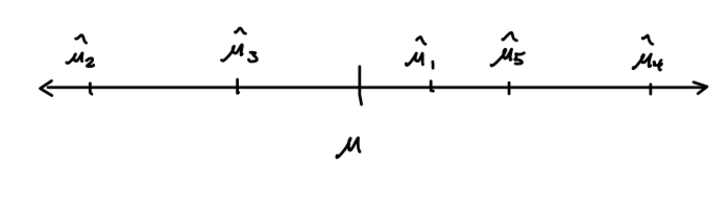
\includegraphics[width=0.5\textwidth]{figures/pop-sample-mean}
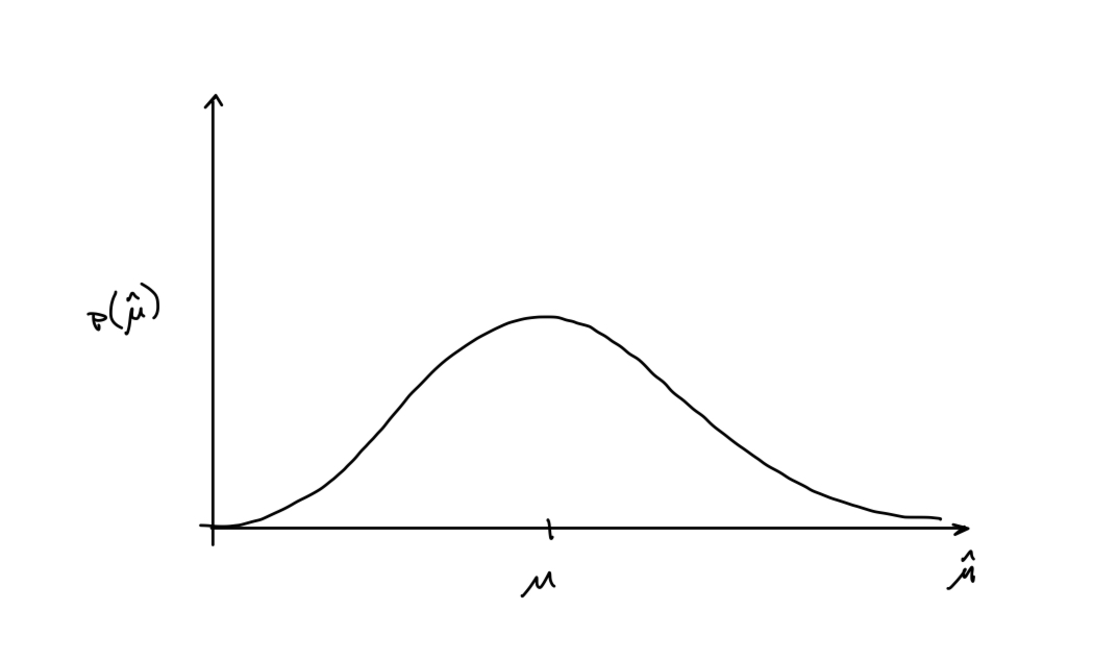
\includegraphics[width=0.5\textwidth]{figures/distribution}
\end{figure}

You get many different values, and in general they will be normally distributed.

\end{frame}

\begin{frame}{Standard error of the mean}

If the sampling process is \textit{unbiased}:
\begin{align*}
\text{avg}(\hat{\mu}) - \mu &= 0\\
\text{var}(\hat{\mu}) = \frac{\sigma^2}{n} &\onslide<2->{\equiv \text{SE}(\hat{\mu})^2}
\end{align*}

\pause
$\sigma$ is the variance of $\epsilon$, i.e. the changes in $y$ that are not correlated with $x$ \textit{across the entire population}.

\vspace{5mm}

\end{frame}

\begin{frame}{Population variance}

Of course we rarely have the population variance.  
\begin{itemize}
\item We don't usually know the true model
\item We don't usually sample the whole population
\end{itemize}

\vspace{5mm}

Instead we use

\begin{align*}
\hat{\text{SE}}(\hat{\mu})^2 = \hat{\sigma}^2\frac{1}{n} = \frac{\text{RSS}}{(n-1)}\frac{1}{n}
\end{align*}
\end{frame}

\begin{frame}{How do we interpret the standard error of the mean?}

In words: it is an estimate of the variance of the sample means, if we were to repeatedly sample.

\pause
\begin{figure}
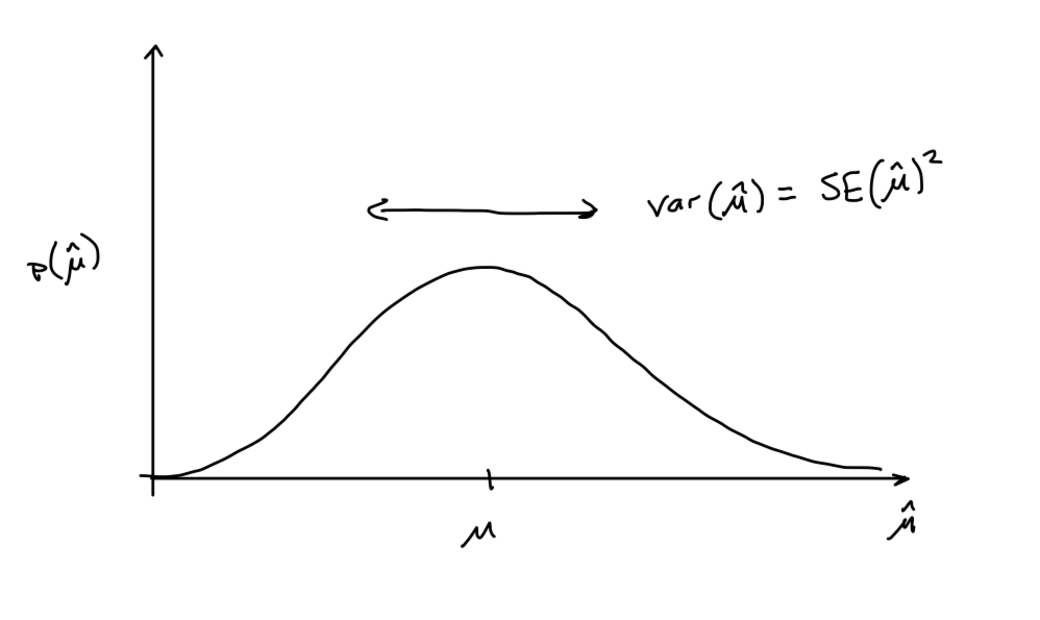
\includegraphics[width=0.5\textwidth]{figures/sample_mean_dist}
\end{figure}

This will be really useful in constructing ``confidence intervals'', in just a few slides.
\end{frame}


\begin{frame}{Ordinary least squares coefficients}

\begin{align*}
y_i=\hat{\beta}_0+\hat{\beta}_1x_i+e_i
\end{align*}
We can think of the coefficients $\hat{\beta}_0$ and $\hat{\beta}_1$ in the same conceptual terms as the sample means.

\begin{align*}
\text{avg}(\hat{\beta}_0) - \beta_0 &= 0\quad\text{(unbiased)}\\
\text{SE}(\hat{\beta}_0)^2 &= \hat{\sigma}^2 \left[ \frac{1}{n} +
\frac{\bar{x}}{\sum_{i=1}^n (x_i-\bar{x})^2} \right]\\
\text{avg}(\hat{\beta}_{1}) - \beta_1 &= 0\quad\text{(unbiased)}\\
\text{SE}(\hat{\beta}_1)^2& = \frac{\hat{\sigma}^2}{\sum_{i=1}^n (x_i-\bar{x})^2}
\end{align*}

\end{frame}

\begin{frame}{Confidence intervals}

For a normal distribution:

\begin{align*}
\text{mean} \pm 2 (\text{standard deviation}) = \mu \pm 2\sigma
\end{align*}

is...\pause the region containing 95\% of the probability mass in the distribution.  

\vspace{5mm}

Therefore the 95\% ``confidence intervals'' are

\begin{align*}
\hat{\beta}_0 \pm 2\text{SE}(\hat{\beta}_0) \\
\hat{\beta}_1 \pm 2\text{SE}(\hat{\beta}_1) 
\end{align*}

If certain conditions are met (we'll cover Thursday) then 
\end{frame}

\begin{frame}{How to interpret the confidence interval?}

\pause

There is a 95\% probability that the ``true'' model coefficient lies within the 95\% confidence interval around the estimated coefficient.  

\vspace{5mm}

Let's explore this concept with an in-class Jupyter notebook.

\vspace{5mm}

  See ``lecture\_09\_supporting.ipynb'' in the ``supporting notebooks'' directory for this lecture.


\end{frame}

\end{document}


